\documentclass{standalone}
\usepackage{tikz}
\usetikzlibrary{patterns, positioning}
\usepackage[sfdefault]{ClearSans} %% option 'sfdefault' activates Clear Sans as the default text font
\usepackage[T1]{fontenc}

\begin{document}
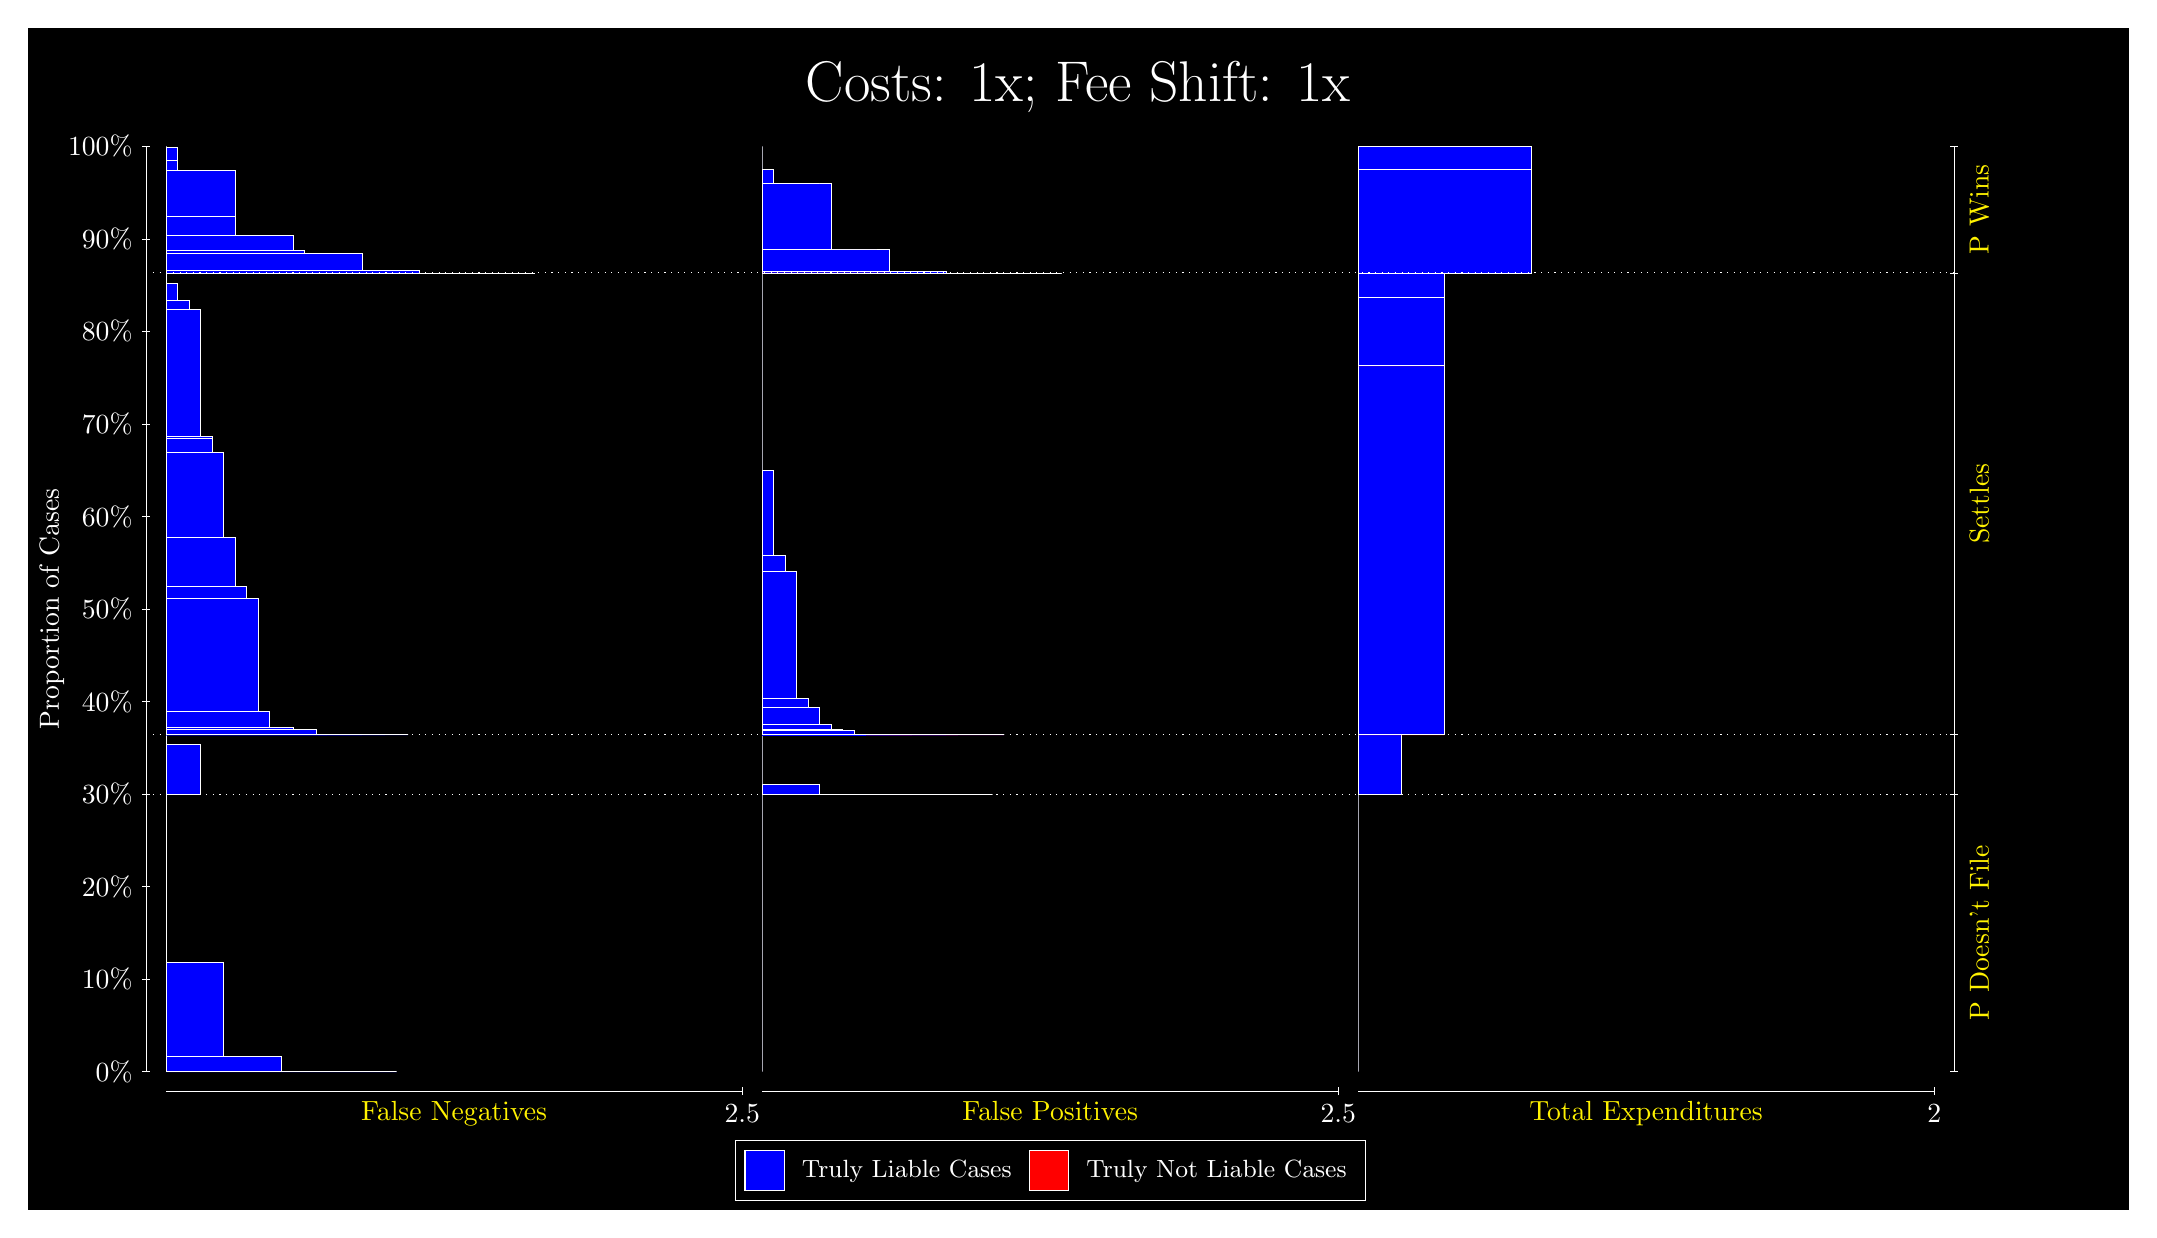
\begin{tikzpicture}
\draw[fill=black] (0,0) rectangle (26.667,15);
\draw[text=white] (0,13.5) rectangle (26.667,15) node[midway] {\huge Costs: 1x; Fee Shift: 1x};
\draw[white, very thin] (1.5,1.75) -- (1.5,13.5);
\node[rotate=90, text=white, anchor=center] at (0.3, 7.625) {Proportion of Cases};
\draw[white, very thin] (1.45,1.75) -- (1.55,1.75);
\node[text=white, anchor=east] at (1.45, 1.75) {0\%};
\draw[white, very thin] (1.45,2.925) -- (1.55,2.925);
\node[text=white, anchor=east] at (1.45, 2.925) {10\%};
\draw[white, very thin] (1.45,4.1) -- (1.55,4.1);
\node[text=white, anchor=east] at (1.45, 4.1) {20\%};
\draw[white, very thin] (1.45,5.275) -- (1.55,5.275);
\node[text=white, anchor=east] at (1.45, 5.275) {30\%};
\draw[white, very thin] (1.45,6.45) -- (1.55,6.45);
\node[text=white, anchor=east] at (1.45, 6.45) {40\%};
\draw[white, very thin] (1.45,7.625) -- (1.55,7.625);
\node[text=white, anchor=east] at (1.45, 7.625) {50\%};
\draw[white, very thin] (1.45,8.8) -- (1.55,8.8);
\node[text=white, anchor=east] at (1.45, 8.8) {60\%};
\draw[white, very thin] (1.45,9.975) -- (1.55,9.975);
\node[text=white, anchor=east] at (1.45, 9.975) {70\%};
\draw[white, very thin] (1.45,11.15) -- (1.55,11.15);
\node[text=white, anchor=east] at (1.45, 11.15) {80\%};
\draw[white, very thin] (1.45,12.325) -- (1.55,12.325);
\node[text=white, anchor=east] at (1.45, 12.325) {90\%};
\draw[white, very thin] (1.45,13.5) -- (1.55,13.5);
\node[text=white, anchor=east] at (1.45, 13.5) {100\%};

\draw[white, very thin] (24.457,1.75) -- (24.457,13.5);
\draw[white, very thin] (24.407,1.75) -- (24.507,1.75);
\node[anchor=west] at (24.407, 1.75) {};
\draw[white, very thin] (24.407,5.2709) -- (24.507,5.2709);
\node[anchor=west] at (24.407, 5.2709) {};
\draw[white, very thin] (24.407,6.0283) -- (24.507,6.0283);
\node[anchor=west] at (24.407, 6.0283) {};
\draw[white, very thin] (24.407,11.892) -- (24.507,11.892);
\node[anchor=west] at (24.407, 11.892) {};
\draw[white, very thin] (24.407,13.5) -- (24.507,13.5);
\node[anchor=west] at (24.407, 13.5) {};

\draw[white, very thin, fill=blue] (1.75,1.75) rectangle (4.6775,1.75);
\draw[white, very thin, fill=blue] (1.75,1.75) rectangle (3.9457,1.7516);
\draw[white, very thin, fill=blue] (1.75,1.7516) rectangle (3.2138,1.9444);
\draw[white, very thin, fill=blue] (1.75,1.9444) rectangle (2.4819,3.1387);
\draw[white, very thin, fill=red] (1.75,3.1387) rectangle (1.75,3.1387);
\draw[white, very thin, fill=blue] (1.75,3.1387) rectangle (1.75,5.2709);
\draw[white, very thin, fill=blue] (1.75,5.2709) rectangle (2.1891,5.9044);
\draw[white, very thin, fill=red] (1.75,5.9044) rectangle (1.75,5.9044);
\draw[white, very thin, fill=blue] (1.75,5.9044) rectangle (1.75,6.0283);
\draw[white, very thin, fill=blue] (1.75,6.0283) rectangle (4.8239,6.0283);
\draw[white, very thin, fill=blue] (1.75,6.0283) rectangle (4.5312,6.0283);
\draw[white, very thin, fill=blue] (1.75,6.0283) rectangle (4.2384,6.0283);
\draw[white, very thin, fill=blue] (1.75,6.0283) rectangle (4.092,6.0283);
\draw[white, very thin, fill=blue] (1.75,6.0283) rectangle (3.7993,6.0283);
\draw[white, very thin, fill=blue] (1.75,6.0283) rectangle (3.6529,6.0977);
\draw[white, very thin, fill=blue] (1.75,6.0977) rectangle (3.5065,6.099);
\draw[white, very thin, fill=blue] (1.75,6.099) rectangle (3.3602,6.126);
\draw[white, very thin, fill=blue] (1.75,6.126) rectangle (3.0674,6.3253);
\draw[white, very thin, fill=blue] (1.75,6.3253) rectangle (3.0674,6.3268);
\draw[white, very thin, fill=blue] (1.75,6.3268) rectangle (2.921,7.7577);
\draw[white, very thin, fill=blue] (1.75,7.7577) rectangle (2.7746,7.909);
\draw[white, very thin, fill=blue] (1.75,7.909) rectangle (2.6283,8.5388);
\draw[white, very thin, fill=blue] (1.75,8.5388) rectangle (2.4819,9.6128);
\draw[white, very thin, fill=blue] (1.75,9.6128) rectangle (2.3355,9.7918);
\draw[white, very thin, fill=blue] (1.75,9.7918) rectangle (2.3355,9.82);
\draw[white, very thin, fill=blue] (1.75,9.82) rectangle (2.1891,11.425);
\draw[white, very thin, fill=blue] (1.75,11.425) rectangle (2.0428,11.549);
\draw[white, very thin, fill=blue] (1.75,11.549) rectangle (1.8964,11.761);
\draw[white, very thin, fill=red] (1.75,11.761) rectangle (1.75,11.761);
\draw[white, very thin, fill=blue] (1.75,11.761) rectangle (1.75,11.892);
\draw[white, very thin, fill=blue] (1.75,11.892) rectangle (6.4341,11.892);
\draw[white, very thin, fill=blue] (1.75,11.892) rectangle (5.7022,11.893);
\draw[white, very thin, fill=blue] (1.75,11.893) rectangle (4.9703,11.925);
\draw[white, very thin, fill=blue] (1.75,11.925) rectangle (4.8239,11.925);
\draw[white, very thin, fill=blue] (1.75,11.925) rectangle (4.2384,12.143);
\draw[white, very thin, fill=blue] (1.75,12.143) rectangle (4.092,12.143);
\draw[white, very thin, fill=blue] (1.75,12.143) rectangle (3.5065,12.18);
\draw[white, very thin, fill=blue] (1.75,12.18) rectangle (3.3602,12.364);
\draw[white, very thin, fill=blue] (1.75,12.364) rectangle (2.7746,12.364);
\draw[white, very thin, fill=blue] (1.75,12.364) rectangle (2.6283,12.611);
\draw[white, very thin, fill=blue] (1.75,12.611) rectangle (2.6283,13.196);
\draw[white, very thin, fill=blue] (1.75,13.196) rectangle (2.0428,13.196);
\draw[white, very thin, fill=blue] (1.75,13.196) rectangle (1.8964,13.324);
\draw[white, very thin, fill=blue] (1.75,13.324) rectangle (1.8964,13.484);
\draw[white, very thin, fill=red] (1.75,13.484) rectangle (1.75,13.484);
\draw[white, very thin, fill=blue] (1.75,13.484) rectangle (1.75,13.5);
\draw[white, very thin, fill=red] (9.3189,1.75) rectangle (9.3189,1.75);
\draw[white, very thin, fill=blue] (9.3189,1.75) rectangle (9.3189,5.2709);
\draw[white, very thin, fill=red] (9.3189,5.2709) rectangle (12.246,5.2709);
\draw[white, very thin, fill=blue] (9.3189,5.2709) rectangle (12.246,5.2709);
\draw[white, very thin, fill=blue] (9.3189,5.2709) rectangle (11.515,5.2709);
\draw[white, very thin, fill=blue] (9.3189,5.2709) rectangle (10.783,5.2719);
\draw[white, very thin, fill=blue] (9.3189,5.2719) rectangle (10.051,5.3948);
\draw[white, very thin, fill=blue] (9.3189,5.3948) rectangle (9.3189,6.0283);
\draw[white, very thin, fill=red] (9.3189,6.0283) rectangle (12.393,6.0283);
\draw[white, very thin, fill=blue] (9.3189,6.0283) rectangle (12.393,6.0283);
\draw[white, very thin, fill=red] (9.3189,6.0283) rectangle (11.807,6.0283);
\draw[white, very thin, fill=blue] (9.3189,6.0283) rectangle (11.807,6.0283);
\draw[white, very thin, fill=blue] (9.3189,6.0283) rectangle (11.661,6.0283);
\draw[white, very thin, fill=red] (9.3189,6.0283) rectangle (11.222,6.0283);
\draw[white, very thin, fill=blue] (9.3189,6.0283) rectangle (11.222,6.0283);
\draw[white, very thin, fill=blue] (9.3189,6.0283) rectangle (11.075,6.0283);
\draw[white, very thin, fill=blue] (9.3189,6.0283) rectangle (10.929,6.0284);
\draw[white, very thin, fill=red] (9.3189,6.0284) rectangle (10.636,6.0284);
\draw[white, very thin, fill=blue] (9.3189,6.0284) rectangle (10.636,6.0287);
\draw[white, very thin, fill=blue] (9.3189,6.0287) rectangle (10.49,6.088);
\draw[white, very thin, fill=red] (9.3189,6.088) rectangle (10.344,6.088);
\draw[white, very thin, fill=blue] (9.3189,6.088) rectangle (10.344,6.0918);
\draw[white, very thin, fill=blue] (9.3189,6.0918) rectangle (10.197,6.1597);
\draw[white, very thin, fill=red] (9.3189,6.1597) rectangle (10.051,6.1597);
\draw[white, very thin, fill=blue] (9.3189,6.1597) rectangle (10.051,6.3713);
\draw[white, very thin, fill=blue] (9.3189,6.3713) rectangle (9.9044,6.4956);
\draw[white, very thin, fill=blue] (9.3189,6.4956) rectangle (9.758,8.1006);
\draw[white, very thin, fill=blue] (9.3189,8.1006) rectangle (9.6116,8.3078);
\draw[white, very thin, fill=blue] (9.3189,8.3078) rectangle (9.4652,9.3818);
\draw[white, very thin, fill=blue] (9.3189,9.3818) rectangle (9.3189,11.892);
\draw[white, very thin, fill=red] (9.3189,11.892) rectangle (13.125,11.892);
\draw[white, very thin, fill=blue] (9.3189,11.892) rectangle (13.125,11.892);
\draw[white, very thin, fill=red] (9.3189,11.892) rectangle (12.393,11.892);
\draw[white, very thin, fill=blue] (9.3189,11.892) rectangle (12.393,11.892);
\draw[white, very thin, fill=red] (9.3189,11.892) rectangle (11.661,11.892);
\draw[white, very thin, fill=blue] (9.3189,11.892) rectangle (11.661,11.908);
\draw[white, very thin, fill=red] (9.3189,11.908) rectangle (10.929,11.908);
\draw[white, very thin, fill=blue] (9.3189,11.908) rectangle (10.929,12.196);
\draw[white, very thin, fill=red] (9.3189,12.196) rectangle (10.783,12.196);
\draw[white, very thin, fill=blue] (9.3189,12.196) rectangle (10.783,12.196);
\draw[white, very thin, fill=blue] (9.3189,12.196) rectangle (10.197,13.028);
\draw[white, very thin, fill=red] (9.3189,13.028) rectangle (10.051,13.028);
\draw[white, very thin, fill=blue] (9.3189,13.028) rectangle (10.051,13.028);
\draw[white, very thin, fill=blue] (9.3189,13.028) rectangle (9.4652,13.212);
\draw[white, very thin, fill=red] (9.3189,13.212) rectangle (9.3189,13.212);
\draw[white, very thin, fill=blue] (9.3189,13.212) rectangle (9.3189,13.5);
\draw[white, very thin, fill=red] (16.888,1.75) rectangle (16.888,1.75);
\draw[white, very thin, fill=blue] (16.888,1.75) rectangle (16.888,5.2709);
\draw[white, very thin, fill=red] (16.888,5.2709) rectangle (17.437,5.2709);
\draw[white, very thin, fill=blue] (16.888,5.2709) rectangle (17.437,6.0283);
\draw[white, very thin, fill=red] (16.888,6.0283) rectangle (17.986,6.0283);
\draw[white, very thin, fill=blue] (16.888,6.0283) rectangle (17.986,10.715);
\draw[white, very thin, fill=red] (16.888,10.715) rectangle (17.986,10.715);
\draw[white, very thin, fill=blue] (16.888,10.715) rectangle (17.986,11.583);
\draw[white, very thin, fill=red] (16.888,11.583) rectangle (17.986,11.583);
\draw[white, very thin, fill=blue] (16.888,11.583) rectangle (17.986,11.892);
\draw[white, very thin, fill=red] (16.888,11.892) rectangle (19.083,11.892);
\draw[white, very thin, fill=blue] (16.888,11.892) rectangle (19.083,13.212);
\draw[white, very thin, fill=red] (16.888,13.212) rectangle (19.083,13.212);
\draw[white, very thin, fill=blue] (16.888,13.212) rectangle (19.083,13.5);
\draw[white, dotted] (1.5,5.2709) -- (24.457,5.2709);
\draw[white, dotted] (1.5,6.0283) -- (24.457,6.0283);
\draw[white, dotted] (1.5,11.892) -- (24.457,11.892);
\draw[white, very thin] (1.75,1.5) -- (9.0689,1.5);
\node[text=yellow, anchor=north] at (5.4094, 1.5) {False Negatives};
\draw[white, very thin] (9.0689,1.45) -- (9.0689,1.55);
\node[text=white, anchor=north] at (9.0689, 1.45) {2.5};

\draw[white, very thin] (9.3189,1.5) -- (16.638,1.5);
\node[text=yellow, anchor=north] at (12.978, 1.5) {False Positives};
\draw[white, very thin] (16.638,1.45) -- (16.638,1.55);
\node[text=white, anchor=north] at (16.638, 1.45) {2.5};

\draw[white, very thin] (16.888,1.5) -- (24.207,1.5);
\node[text=yellow, anchor=north] at (20.547, 1.5) {Total Expenditures};
\draw[white, very thin] (24.207,1.45) -- (24.207,1.55);
\node[text=white, anchor=north] at (24.207, 1.45) {2};

\node[text=yellow, centered, rotate=90] at (24.777, 3.5105) {P Doesn't File};

\node[text=yellow, centered, rotate=90] at (24.777, 8.9603) {Settles};
\node[text=yellow, centered, rotate=90] at (24.777, 12.696) {P Wins};

\draw (12.978300999999998,1.5) node[draw=none] (baseCoordinate) {};
\begin{scope}[align=center]
        \matrix[scale=0.5, draw=white, below=0.5cm of baseCoordinate, nodes={draw}, column sep=0.1cm]{
            \node[rectangle, draw, minimum width=0.5cm, minimum height=0.5cm, fill=blue] {}; &
            \node[draw=none, font=\small, text=white] (B) {Truly Liable Cases}; &
            \node[rectangle, draw, minimum width=0.5cm, minimum height=0.5cm, fill=red] {}; &
            \node[draw=none, font=\small, text=white] (B) {Truly Not Liable Cases}; \\
            };
\end{scope}

\end{tikzpicture}
\end{document}